% ===========================================================================
%
%		FEDERICO II THESIS TEMPLATE - ENGLISH
%  					* an example of Chapter 1: information about the discussion of the thesis
%	 
% 		AUTHOR:  		Antonio Esposito (antonio.esposito103@studenti.unina.it)
%		LAST UPDATED:	2017/06/20
%
% ===========================================================================
\chapter{Introduzione}
Lo scopo di questo documento è quello di specificare i requisiti del sistema software "Cerca Viaggi" per facilitarne la realizzazione e la validazione ed, in particolare,
si vogliono formalizzare i requisiti funzionali e non funzionali del sistema. \\Il documento prevede vari livelli di raffinamento partendo dal linguaggio naturale
ed arrivando ad un linguaggio strutturato ed a modelli UML.
\section{Requisiti Funzionali}
\begin{enumerate}
    \item  \textbf{Accesso amministratore al sistema}: un amministratore dovrà poter accedere al sistema tramite email e password (usando l'applicativo dekstop).
    \item  \textbf{Amministratore valuta una recensione}: un amministatore dovrà poter accettare o rifiutare una recensione scritta da un utente decidendo quindi se questa verrà pubblicata o eliminata.
    \item \textbf{Accesso utente al sistema}: un utente, dopo aver effettuato la registrazione, dovrà poter accedere al suo account tramite email e password (usando l'applicativo mobile). 
    \item  \textbf{Registrazione di un nuovo utente}: l'applicativo mobile dovrà permettere ad un utente, non precedentemente registrato, di creare un account specificando 
    i propri dati anagrafici (nome, cognome e data di nascita), i dati per effettuare l'accesso (email e passowrd) ed un nickname da utilizzare, secondo volonta dell'utente, per firmare  
    le proprie recensioni
    \item \textbf{Amministratore modifica dati dei visitatori}: un amministratore dovrà poter modificare i dati di un utente in particolare, email e password
    \item \textbf{Amministratore elimina account utente}: un amministratore dovrà poter eliminare l'account di un utente
    \item \textbf{Amministratore visualizza dati di un visitatore}: un amministratore dovrà poter visualizzare i dati anagrafici di un visitatore (nome, cognome e data di nascita), 
    il nickname ed il numero di recensioni approvate e rifiutate.
    \item \textbf{Utente visualizza struttra}: un utente dovrà poter visualizzare i dettagli di una struttura dopo averla selezionata.
    \item \textbf{Utente scrive una recensione}: un utente, una volta aver effettuato l'accesso, dovrà poter scrivere una recensione ad una struttura.
    \item \textbf{Utente visualizaza dettagli recensione}: un utente dovrà poter leggere i dettagli di una recensione, in particolare leggendone l'autore, la data di inserimento, la valutazione
    ed il testo integrale.
    \item \textbf{Utente ricerca una struttura}: un utente dovrà poter ricercare una struttura in vari modi: per nome, tramite filtri (fascia di prezzo, distanza massima dalla posizione attuale, 
    città e categoria) o tramite l'ausilio della mappa.
\end{enumerate}
\section{Requisiti non funzionali}
\begin{enumerate}
    \item Il sistema deve garantire una buona usabilità per tutti coloro che ne usufruiscono.
\end{enumerate}
\chapter{Modello funzionale}

%%%%% ===============================================================================
\section{Modellazione dei casi d'uso}

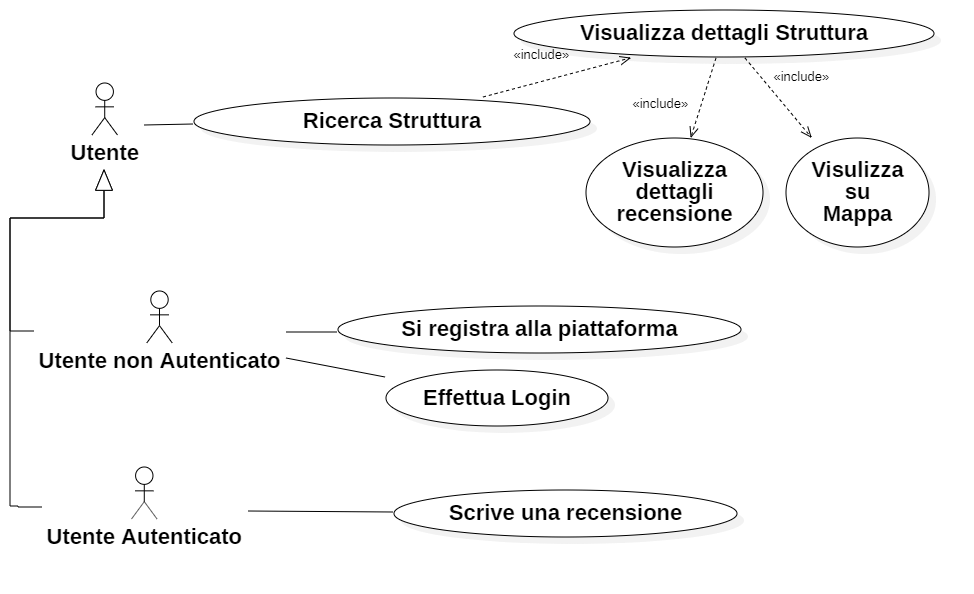
\includegraphics[scale=0.4]{Usecase/ucd2.png}
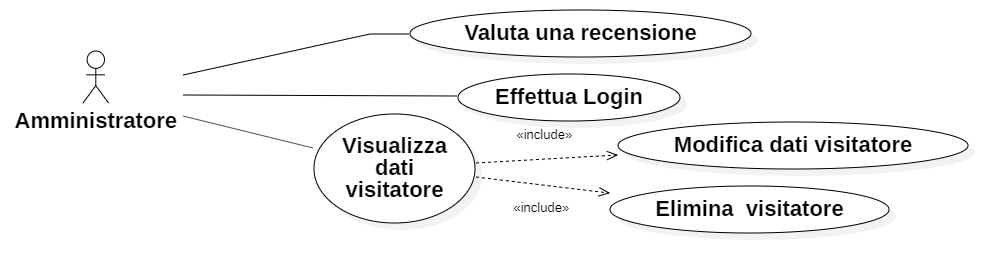
\includegraphics[scale=0.4]{Usecase/ucd1.png}


%%%%% ===============================================================================
\section{Tabelle di Cockburn}


\begin{table}[h!]    
\def\arraystretch{1.5}
\caption{L'amministratore effettua il login }

%Intestazione tabella%
\begin{tabularx}{\textwidth}{|l|X|X|X|X|}
 \rowcolor{Gray}
  \hline Use Case \#1 & \multicolumn{4} {l|}{Effettua Login} \\ \hline Goal in
  Context & \multicolumn{4}{>{\hsize=\dimexpr 4\hsize+4\tabcolsep+2\arrayrulewidth\relax}X|}{%
    L'amministratore vuole accedere all'applicativo di Back-Office} \\
 \hline Preconditions & \multicolumn{4}{>{\hsize=\dimexpr 4\hsize+4\tabcolsep+2\arrayrulewidth\relax}X|}{%
 L'amministratore non ha effettuto lo use case "Effettua Login".  } \\
 \hline Success End Conditions &
 \multicolumn{4}{>{\hsize=\dimexpr 4\hsize+4\tabcolsep+2\arrayrulewidth\relax}X|}{ Il login dell'amministratore va a buon fine.} \\
 \hline Failed End Conditions &
 \multicolumn{4}{>{\hsize=\dimexpr 4\hsize+4\tabcolsep+2\arrayrulewidth\relax}X|}{I dati di login sono errati o il server non è raggiungibile.} \\
 \hline Primary Actor &
  \multicolumn{4}{l|}{Amministratore} \\
 \hline Trigger & 
 \multicolumn{4}{>{\hsize=\dimexpr 4\hsize+4\tabcolsep+2\arrayrulewidth\relax}X|}{L'amministratore preme il pulsante "Login" nella schermata LoginForm visibile all'avvio del software.} \\
\hline
%Main Scenario%
\multicolumn{5}{|>{\hsize=\dimexpr 4\hsize+4\tabcolsep+2\arrayrulewidth\relax}c|}{Main Scenario}\\\hline
\end{tabularx}
\setlength{\tabcolsep}{8pt}
\renewcommand{\arraystretch}{1.5}
    \begin{tabularx}{\textwidth}{|c|X|X|}
        Step\# & Amministratore & Sistema \\
        \hline
         1 &Compila correttamente i textField Username e Password  & \\
         \hline
         2 &Preme il pulsante "Login" dalla schermata LoginForm  & \\
         \hline
         3 &  &Mostra schermata HomePage\\
        \hline
    \end{tabularx} 
    \end{table}
    \begin{table}[H]
        \caption{Effettua Login - Estensione 1}
    %Extension 1%
    \begin{tabularx}{\textwidth}{|c|X|X|}
            \hline
            \rowcolor{LightGray}
            \multicolumn{3}{|>{\hsize=\dimexpr 4\hsize+4\tabcolsep+2\arrayrulewidth\relax}c|}{Extension 1: l'amministatore inserisce dati errati}\\\hline
            Step\# & Amministratore & Sistema \\
            \hline
             1 a &  Non complia o compila erroneamente i textField Username e Password& \\
             \hline
             2 a & Preme il pulsante Login & \\
             \hline
             3 a & & Mostra CredenzialiErrateDialog \\
             \hline
             4 a & Preme il tasto Ok&  \\
             \hline
             5 a & & Mostra LoginForm e termina caso d'uso\\
             \hline        
        \end{tabularx} 
    \end{table}
    \begin{table}[h!]
        \caption{Effettua Login - Estensione 2}
    %Extension 2%
    \begin{tabularx}{\textwidth}{|c|X|X|}
        \hline
        \rowcolor{LightGray}
        \multicolumn{3}{|>{\hsize=\dimexpr 4\hsize+4\tabcolsep+2\arrayrulewidth\relax}c|}{Extension 2: il server non è raggiungibile}\\\hline
        Step\# & Amministratore & Sistema \\
        \hline
         1 b &  Compila i campi username e password& \\
         \hline
         2 b & Preme il pulsante Login & \\
         \hline
         3 a & & Mostra 'Connessione assente dialog' e termina caso d'uso \\
         \hline
       
    \end{tabularx} 
\end{table}


\begin{table}[H]    
\def\arraystretch{1.5}
\caption{L'amministratore valuta una recensione}

%Intestazione tabella%
\begin{tabularx}{\textwidth}{|l|X|X|X|X|}
  \rowcolor{Gray}
  \hline Use Case \#2 & \multicolumn{4} {l|}{Valuta Recensione} \\ \hline Goal in
  Context & \multicolumn{4}{>{\hsize=\dimexpr 4\hsize+4\tabcolsep+2\arrayrulewidth\relax}X|}{%
    L'amministratore valuta una recensione.} \\
 \hline Preconditions & \multicolumn{4}{>{\hsize=\dimexpr 4\hsize+4\tabcolsep+2\arrayrulewidth\relax}X|}{%
 L'amministratore ha effettuto lo use case "Effettua Login".  } \\
 \hline Success End Conditions &
 \multicolumn{4}{>{\hsize=\dimexpr 4\hsize+4\tabcolsep+2\arrayrulewidth\relax}X|}{ L'amministratore valuta una recensione. Il sistema tiene traccia di tale operazione.} \\
 \hline Failed End Conditions &
 \multicolumn{4}{>{\hsize=\dimexpr 4\hsize+4\tabcolsep+2\arrayrulewidth\relax}X|}{L'amministatore preme annulla. L'amministrazione valuta una recensione che è già stata valutata. Il server non è raggiungibile.} \\
 \hline Primary Actor &
  \multicolumn{4}{l|}{Amministratore} \\
 \hline Trigger & 
 \multicolumn{4}{>{\hsize=\dimexpr 4\hsize+4\tabcolsep+2\arrayrulewidth\relax}X|}{L'amministratore preme il pulsante "Recensioni" nella Homepage.} \\
\hline
%Main Scenario%
\multicolumn{5}{|>{\hsize=\dimexpr 4\hsize+4\tabcolsep+2\arrayrulewidth\relax}c|}{Main Scenario}\\\hline
\end{tabularx}
\setlength{\tabcolsep}{8pt}
\renewcommand{\arraystretch}{1.5}
    \begin{tabularx}{\textwidth}{|c|X|X|}
        Step\# & Amministratore & Sistema \\
        \hline
         1 &Preme il pulsante "Recensioni" nella schermata principale & \\
         \hline
         2 & & Mostra schermata "Recensioni"\\
         \hline
         3 & Clicca sulla card di una recensione  &\\
         \hline
         4 & & Mostra schermata "Visualizza Recensione"\\
       \hline
         5 & Clicca sul pulsante Accetta &\\
        \hline
        6& &Mostra 'Recensione Approvata Dialog' e termina lo use case\\
        \hline
    \end{tabularx}
    %Subvariation 1%
\end{table}
\begin{table}[h!]
    \caption{Valuta una recensione - Subvariation 1}
        \begin{tabularx}{\textwidth}{|c|X|X|}
            \hline
            \rowcolor{LightGray}
            \multicolumn{3}{|>{\hsize=\dimexpr 4\hsize+4\tabcolsep+2\arrayrulewidth\relax}c|}{Subvariation 1: l'amministatore rifiuta una recensione}\\\hline
            Step\# & Amministratore & Sistema \\
            \hline
             5 i &Preme il pulsante "Rifiuta". & \\
             \hline
             6 i & & Mostra 'Recensione Rifiutata Dialog' e termina lo use case.\\
            \hline
        \end{tabularx}
\setlength{\tabcolsep}{8pt}
\renewcommand{\arraystretch}{1.5}
\end{table}

 %Extension 1%
\begin{table}[h!]
    \caption{Valuta una recensione - Estensione 1}
    \begin{tabularx}{\textwidth}{|c|X|X|}
        \hline
        \rowcolor{LightGray}
        \multicolumn{3}{|>{\hsize=\dimexpr 4\hsize+4\tabcolsep+2\arrayrulewidth\relax}c|}{Extension 1: l'amministatore preme annulla}\\\hline
        Step\# & Amministratore & Sistema \\
        \hline
         3/5 a &Preme il pulsante "Recensioni" dal menu laterale sinistro & \\
         \hline
         4/6 a & & Ritorna alla schermata principale e termina il caso d'uso.\\
        \hline
    \end{tabularx}
\end{table}
%Estensione 2
\begin{table}[h!]
    \caption{Valuta una recensione - Estensione 2}
     \begin{tabularx}{\textwidth}{|c|X|X|}
        \hline
        \rowcolor{LightGray}
        \multicolumn{3}{|>{\hsize=\dimexpr 4\hsize+4\tabcolsep+2\arrayrulewidth\relax}c|}{Extension 2: la recensione è già stata valutata }\\\hline
         Step\# & Amministratore & Sistema \\
         \hline
          4 b  & & Mostra Fallimento Dialog e termina caso d'uso \\
          \hline
     \end{tabularx}
\end{table}
%Estensione 3
\begin{table}[h!]
    \caption{Valuta una recensione - Estensione 3}
     \begin{tabularx}{\textwidth}{|c|X|X|}
        \hline
        \rowcolor{LightGray}
        \multicolumn{3}{|>{\hsize=\dimexpr 4\hsize+4\tabcolsep+2\arrayrulewidth\relax}c|}{Extension 3: il server non è raggiungibile }\\\hline
         Step\# & Amministratore & Sistema \\
         \hline
          4/6 c  & & Mostra Connessione Assente Dialog e termina caso d'uso \\
          \hline
     \end{tabularx}
\end{table}
\pagebreak
\pagebreak
\begin{table}[H]    
    \def\arraystretch{1.5}
    \caption{L'amministratore visualizza dati di un visitatore}
    
    %Intestazione tabella%
    \begin{tabularx}{\textwidth}{|l|X|X|X|X|}
        \rowcolor{Gray}
      \hline Use Case \#3 & \multicolumn{4} {l|}{Visualizza dati visitatore} \\ \hline Goal in
      Context & \multicolumn{4}{>{\hsize=\dimexpr 4\hsize+4\tabcolsep+2\arrayrulewidth\relax}X|}{%
        L'amministratore visualizza i dati di un visitatore.} \\
     \hline Preconditions & \multicolumn{4}{>{\hsize=\dimexpr 4\hsize+4\tabcolsep+2\arrayrulewidth\relax}X|}{%
     L'amministratore ha effettuto lo use case "Effettua Login".  } \\
     \hline Success End Conditions &
     \multicolumn{4}{>{\hsize=\dimexpr 4\hsize+4\tabcolsep+2\arrayrulewidth\relax}X|}{ L'amministratore visualizza con successo i dati di un visitatore} \\
     \hline Failed End Conditions &
     \multicolumn{4}{>{\hsize=\dimexpr 4\hsize+4\tabcolsep+2\arrayrulewidth\relax}X|}{Il server non è raggiungibile} \\
     \hline Primary Actor &
      \multicolumn{4}{l|}{Amministratore} \\
     \hline Trigger & 
     \multicolumn{4}{>{\hsize=\dimexpr 4\hsize+4\tabcolsep+2\arrayrulewidth\relax}X|}{L'amministratore preme il pulsante "Visitatori" a partire dalla Schermata "Recensioni" .} \\
    \hline
    %Main Scenario%
    \multicolumn{5}{|>{\hsize=\dimexpr 4\hsize+4\tabcolsep+2\arrayrulewidth\relax}c|}{Main Scenario}\\\hline
    \end{tabularx}
\end{table}
\begin{table}[h!]
    \setlength{\tabcolsep}{8pt}
    \renewcommand{\arraystretch}{1.5}
        \begin{tabularx}{\textwidth}{|c|X|X|}
            \hline
            Step\# & Amministratore & Sistema \\
            \hline
             1 &Preme sul rigo corrispondente all'utente da visualizzare & \\
             \hline
             2 & & Mostra schermata "Visualizza Visitatore" e termina caso d'uso\\
             \hline
        \end{tabularx}
        %Extension 1%
\end{table}
    \begin{table}[h!]
        \caption{Visualizza dati visitatore - Estensione 1}
            \begin{tabularx}{\textwidth}{|c|X|X|}
                \hline
                \rowcolor{LightGray}
                \multicolumn{3}{|>{\hsize=\dimexpr 4\hsize+4\tabcolsep+2\arrayrulewidth\relax}c|}{Extension 1: il server non è raggiungibile}\\\hline
                Step\# & Amministratore & Sistema \\
                \hline
             1 &Preme sul rigo corrispondente all'utente da visualizzare & \\
             \hline
             2 & & Mostra schermata "Connessione assente" e termina caso d'uso\\
             \hline
            \end{tabularx}
    \end{table}
    
    
\pagebreak
\begin{table}[H]    
    \def\arraystretch{1.5}
    \caption{L'amministratore modifica i dati di un visitatore}
    
    %Intestazione tabella%
    \begin{tabularx}{\textwidth}{|l|X|X|X|X|}
        \rowcolor{Gray}
      \hline Use Case \#4 & \multicolumn{4} {l|}{Modifica i dati visitatore} \\ \hline Goal in
      Context & \multicolumn{4}{>{\hsize=\dimexpr 4\hsize+4\tabcolsep+2\arrayrulewidth\relax}X|}{%
        L'amministratore vuole modificare lo username e la password di un visitatore} \\
     \hline Preconditions & \multicolumn{4}{>{\hsize=\dimexpr 4\hsize+4\tabcolsep+2\arrayrulewidth\relax}X|}{%
     L'amministratore ha effettuto lo use case "Effettua Login".  } \\
     \hline Success End Conditions &
     \multicolumn{4}{>{\hsize=\dimexpr 4\hsize+4\tabcolsep+2\arrayrulewidth\relax}X|}{ L'amministratore modifica con successo i dati di un visitatore} \\
     \hline Failed End Conditions &
     \multicolumn{4}{>{\hsize=\dimexpr 4\hsize+4\tabcolsep+2\arrayrulewidth\relax}X|}{Il server non è raggiungibile o l'amministratore non compila correttamente tutti i campi} \\
     \hline Primary Actor &
      \multicolumn{4}{l|}{Amministratore} \\
     \hline Trigger & 
     \multicolumn{4}{>{\hsize=\dimexpr 4\hsize+4\tabcolsep+2\arrayrulewidth\relax}X|}{L'amministratore preme il pulsante "Modifica" dalla Schermata "Visualizza Visitatore" .} \\
    \hline
    %Main Scenario%
    \multicolumn{5}{|>{\hsize=\dimexpr 4\hsize+4\tabcolsep+2\arrayrulewidth\relax}c|}{Main Scenario}\\\hline
    \end{tabularx}
\end{table}
\begin{table}[h!]
    \setlength{\tabcolsep}{8pt}
    \renewcommand{\arraystretch}{1.5}
        \begin{tabularx}{\textwidth}{|c|X|X|}
            \rowcolor{Gray}
            \hline
            Step\# & Amministratore & Sistema \\
            \hline
             1 &Preme sul tasto "Modifica" dalla schermata "Visualizza Visitatore" & \\
             \hline
             2 & & Mostra schermata "Modifica Visitatore" \\
             \hline
             3 & Compila correttamente tutti i campi di testo&  \\
             \hline
             4 & Preme il tasto "Conferma" & \\
             \hline
             5 & & Mostra schermata "Modifica Success Dialog" e termina caso d'uso \\
             \hline
        \end{tabularx}
    \end{table}
    %Extension 1%
    \begin{table}[h!]
        \caption{Modifica dati visitatore - Estensione 1}
            \begin{tabularx}{\textwidth}{|c|X|X|}
                \hline
                \rowcolor{LightGray}
                \multicolumn{3}{|>{\hsize=\dimexpr 4\hsize+4\tabcolsep+2\arrayrulewidth\relax}c|}{Extension 1: il server non è raggiungibile}\\\hline
                Step\# & Amministratore & Sistema \\
                \hline
                1a &Preme sul tasto "Modifica" dalla schermata "Visualizza Visitatore" & \\
                \hline
                2a & & Mostra schermata "Connessione Assente Dialog" \\
             \hline
            \end{tabularx}
    \end{table}
    %Extension 2%
    \begin{table}[h!]
        \caption{Modifica dati visitatore - Estensione 2}
            \begin{tabularx}{\textwidth}{|c|X|X|}
                \hline
                \rowcolor{LightGray}
                \multicolumn{3}{|>{\hsize=\dimexpr 4\hsize+4\tabcolsep+2\arrayrulewidth\relax}c|}{Extension 2: l'amministratore compila erroneamente i campi di testo}\\\hline
                Step\# & Amministratore & Sistema \\
                \hline
                3b &Non compila, compila parzialmente o compila in modo errato i campi di testo & \\
                \hline
                2a & & Mostra schermata "Password o username invalidi dialog" \\
             \hline
            \end{tabularx}
    \end{table}
    
    

\begin{table}[H]    
    \def\arraystretch{1.5}
    \caption{L'amministratore elimina un visitatore}
    
    %Intestazione tabella%
    \begin{tabularx}{\textwidth}{|l|X|X|X|X|}
        \rowcolor{Gray}
      \hline Use Case \#5 & \multicolumn{4} {l|}{Elimina un visitatore} \\ \hline Goal in
      Context & \multicolumn{4}{>{\hsize=\dimexpr 4\hsize+4\tabcolsep+2\arrayrulewidth\relax}X|}{%
        L'amministratore vuole eliminare un visitatore} \\
     \hline Preconditions & \multicolumn{4}{>{\hsize=\dimexpr 4\hsize+4\tabcolsep+2\arrayrulewidth\relax}X|}{%
     L'amministratore ha effettuto lo use case "Effettua Login".  } \\
     \hline Success End Conditions &
     \multicolumn{4}{>{\hsize=\dimexpr 4\hsize+4\tabcolsep+2\arrayrulewidth\relax}X|}{ L'amministratore elimina un visitatore ed il sistema tiene traccia di questa azione} \\
     \hline Failed End Conditions &
     \multicolumn{4}{>{\hsize=\dimexpr 4\hsize+4\tabcolsep+2\arrayrulewidth\relax}X|}{Il server non è raggiungibile } \\
     \hline Primary Actor &
      \multicolumn{4}{l|}{Amministratore} \\
     \hline Trigger & 
     \multicolumn{4}{>{\hsize=\dimexpr 4\hsize+4\tabcolsep+2\arrayrulewidth\relax}X|}{L'amministratore preme il pulsante "Elimina" dalla Schermata "Visualizza Visitatore" .} \\
    \hline
    %Main Scenario%
    \multicolumn{5}{|>{\hsize=\dimexpr 4\hsize+4\tabcolsep+2\arrayrulewidth\relax}c|}{Main Scenario}\\\hline
    \end{tabularx}
\end{table}
\begin{table}[h!]
    \setlength{\tabcolsep}{8pt}
    \renewcommand{\arraystretch}{1.5}
        \begin{tabularx}{\textwidth}{|c|X|X|}
            \rowcolor{Gray}
            \hline
            Step\# & Amministratore & Sistema \\
            \hline
             1 &Preme sul tasto "Elimna" dalla schermata "Visualizza Visitatore" & \\
             \hline
             2 & & Mostra schermata "Utente Eliminato Dialog" e termina caso d'uso \\
             \hline
        \end{tabularx}
    \end{table}
    %Extension 1%
    \begin{table}[h!]
        \caption{Elimina visitatore - Estensione 1}
            \begin{tabularx}{\textwidth}{|c|X|X|}
                \hline
                \rowcolor{LightGray}
                \multicolumn{3}{|>{\hsize=\dimexpr 4\hsize+4\tabcolsep+2\arrayrulewidth\relax}c|}{Extension 1: il server non è raggiungibile}\\\hline
                Step\# & Amministratore & Sistema \\
                \hline
                1a &Preme sul tasto "Elimina" dalla schermata "Visualizza Visitatore" & \\
                \hline
                2a & & Mostra schermata "Connessione Assente Dialog" \\
             \hline
            \end{tabularx}
    \end{table}
    
    
\pagebreak

%finito

%Intestazione tabella%
\begin{table}
\begin{tabularx}{\textwidth}{|l|X|X|X|X|}
  \hline Use Case \#1 & \multicolumn{4} {l|}{Utente effettua Login} \\ \hline Goal in
  Context & \multicolumn{4}{>{\hsize=\dimexpr 4\hsize+4\tabcolsep+2\arrayrulewidth\relax}X|}{%
    L'utente non loggato effettua il login} \\
 \hline Preconditions & \multicolumn{4}{>{\hsize=\dimexpr 4\hsize+4\tabcolsep+2\arrayrulewidth\relax}X|}{%
 L'utente non autenticato non ha effettuto lo use case "Utente effettua Login".  } \\
 \hline Success End Conditions &
 \multicolumn{4}{>{\hsize=\dimexpr 4\hsize+4\tabcolsep+2\arrayrulewidth\relax}X|}{ Il login dell'utente va a buon fine.} \\
 \hline Failed End Conditions &
 \multicolumn{4}{>{\hsize=\dimexpr 4\hsize+4\tabcolsep+2\arrayrulewidth\relax}X|}{I dati di login sono errati oppure il server non è raggiungibile.} \\
 \hline Primary Actor &
  \multicolumn{4}{l|}{Utente non loggato} \\
 \hline Trigger & 
 \multicolumn{4}{>{\hsize=\dimexpr 4\hsize+4\tabcolsep+2\arrayrulewidth\relax}X|}{L'utente preme il pulsante 'Login' nel Navigation Drawer laterale dalla schermata 'HomePage utente non loggato'.} \\
\hline
%Main Scenario%
\multicolumn{5}{|>{\hsize=\dimexpr 4\hsize+4\tabcolsep+2\arrayrulewidth\relax}c|}{Main Scenario}\\\hline
\end{tabularx}
\setlength{\tabcolsep}{8pt}
\renewcommand{\arraystretch}{1.5}
    \begin{tabularx}{\textwidth}{|c|X|X|}
        Step\# & Utente & Sistema \\
        \hline
         1 &Compila correttamente i textField Username e Password  & \\
         \hline
         2 &Preme il pulsante "Login" dalla schermata LoginForm  & \\
         \hline
         3 &  &Mostra schermata HomePage\\
        \hline
    \end{tabularx}
    %Extension 1%
        \begin{tabularx}{\textwidth}{|c|X|X|}
            \hline
            \multicolumn{3}{|>{\hsize=\dimexpr 4\hsize+4\tabcolsep+2\arrayrulewidth\relax}c|}{Extension 1: l'utente inserisce dati errati}\\\hline
            Step\# & Utente & Sistema \\
            \hline
             1 a &  Compila erroneamente i textField Username e Password& \\
             \hline
             2 a & Preme il pulsante Login & \\
             \hline
             3 a & & Mostra schermata Login Dati Errati Dialog \\
             \hline
             4 a & Preme il tasto 'Riprova'&  \\
             \hline
             5 a & & Mostra Login e termina caso d'uso\\
             \hline        
        \end{tabularx} 
    %Extension 2%
    \begin{tabularx}{\textwidth}{|c|X|X|}
      \hline
      \multicolumn{3}{|>{\hsize=\dimexpr 4\hsize+4\tabcolsep+2\arrayrulewidth\relax}c|}{Extension 2: l'utente non compila tutti i campi}\\\hline
      Step\# & Utente & Sistema \\
      \hline
       1 b &  Non compila o compila solo un tra i textField Username e Password& \\
       \hline
       2 b & Preme il pulsante Login & \\
       \hline
       3 b & & Mostra schermata Login campi vuoti Dialog \\
       \hline
       4 b & Preme il tasto 'Riprova'&  \\
       \hline
       5 b & & Mostra Login e termina caso d'uso\\
       \hline        
  \end{tabularx}
\end{table}
\pagebreak
%Extension 3%
\begin{table}
\begin{tabularx}{\textwidth}{|c|X|X|}
  \hline
  \multicolumn{3}{|>{\hsize=\dimexpr 4\hsize+4\tabcolsep+2\arrayrulewidth\relax}c|}{Extension 3: il server risulta non raggiungibile}\\\hline
  Step\# & Utente & Sistema \\
  \hline
   3 c & & Mostra schermata Login server irraggiungibile \\
   \hline
   4 c & Preme il tasto 'Riprova'&  \\
   \hline
   5 c & & Mostra Login e termina caso d'uso\\
   \hline        
\end{tabularx} 
\end{table}


%Intestazione tabella%
\begin{table}[h!]
\caption{L'utente non loggato effettua la registazione}
\begin{tabularx}{\textwidth}{|l|X|X|X|X|}
  \hline Use Case \#2 & \multicolumn{4} {l|}{L'utente non loggato si registra alla piattaforma} \\ \hline Goal in
  Context & \multicolumn{4}{>{\hsize=\dimexpr 4\hsize+4\tabcolsep+2\arrayrulewidth\relax}X|}{%
    L'utente non loggato effettua la registrazione} \\
 \hline Preconditions & \multicolumn{4}{>{\hsize=\dimexpr 4\hsize+4\tabcolsep+2\arrayrulewidth\relax}X|}{%
 -  } \\
 \hline Success End Conditions &
 \multicolumn{4}{>{\hsize=\dimexpr 4\hsize+4\tabcolsep+2\arrayrulewidth\relax}X|}{ La registrazione dell'utente va a buon fine.} \\
 \hline Failed End Conditions &
 \multicolumn{4}{>{\hsize=\dimexpr 4\hsize+4\tabcolsep+2\arrayrulewidth\relax}X|}{Il server non è raggiungibile o l'utente immette dati non validi.} \\
 \hline Primary Actor &
  \multicolumn{4}{l|}{Utente non loggato} \\
 \hline Trigger & 
 \multicolumn{4}{>{\hsize=\dimexpr 4\hsize+4\tabcolsep+2\arrayrulewidth\relax}X|}{L'utente preme il pulsante 'Registrati' nel Navigation Drawer laterale dalla schermata 'HomePage utente non loggato'.} \\
\hline
%Main Scenario%
\multicolumn{5}{|>{\hsize=\dimexpr 4\hsize+4\tabcolsep+2\arrayrulewidth\relax}c|}{Main Scenario}\\\hline
\end{tabularx}
\setlength{\tabcolsep}{8pt}
\renewcommand{\arraystretch}{1.5}
    \begin{tabularx}{\textwidth}{|c|X|X|}
        Step\# & Utente & Sistema \\
        \hline
         1 &Compila correttamente tutti i textField ed il date picker  & \\
         \hline
         2 &Preme il pulsante "Fine" dalla schermata Registrazione  & \\
         \hline
         3 &  &Mostra schermata "Registrazione success dialog" e termina il caso d'uso\\
        \hline
    \end{tabularx}
  \end{table}
  \begin{table}[h!]
    \caption{Effettua registrazione - Estensione 1}
    %Extension 1%
        \begin{tabularx}{\textwidth}{|c|X|X|}
            \hline
            \multicolumn{3}{|>{\hsize=\dimexpr 4\hsize+4\tabcolsep+2\arrayrulewidth\relax}c|}{Extension 1: l'utente inserisce dati di un utente già registrato}\\\hline
            Step\# & Utente & Sistema \\
            \hline
             1 a &  Compila i textField inserendo i dati di un account già registrato& \\
             \hline
             2 a & Preme il pulsante "Fine" & \\
             \hline
             3 a & & Mostra schermata "Registrazione utente esistente fail dialog" e termina il caso d'uso\\
             \hline        
        \end{tabularx} 
      \end{table}

    %Extension 2%
    \begin{table}[h!]
    \caption{Effettura registrazione - Estensione 2}
    \begin{tabularx}{\textwidth}{|c|X|X|}
      \hline
      \multicolumn{3}{|>{\hsize=\dimexpr 4\hsize+4\tabcolsep+2\arrayrulewidth\relax}c|}{Extension 2: l'utente non compila tutti i campi o li compila in modo errato}\\\hline
      Step\# & Utente & Sistema \\
      \hline
       1 b &  Non compila o compila erroneamente i textfiel ed il datepicker& \\
       \hline
       2 b & Preme il pulsante "Fine" & \\
       \hline
       3 b & & Mostra schermata "Campi non compilato o errati dialog" e termina caso d'uso  \\
       \hline        
  \end{tabularx}
\end{table}

%Extension 3%
\begin{table}[h!]
  \caption{Effettura registrazione - Estensione 3}
\begin{tabularx}{\textwidth}{|c|X|X|}
  \hline
  \multicolumn{3}{|>{\hsize=\dimexpr 4\hsize+4\tabcolsep+2\arrayrulewidth\relax}c|}{Extension 3: il server risulta non raggiungibile}\\\hline
  Step\# & Utente & Sistema \\
  \hline
  1 c & Compila correttamente tutti i campi della registrazione&  \\
  \hline
  2 c & Preme il tasto "Fine"&  \\
  \hline
  3 c & & Mostra schermata "Registrazione server irraggiungibile" e termina caso d'uso \\
   \hline
\end{tabularx} 
\end{table}


%Intestazione tabella%
\begin{table}[H]
    \caption{L'utente non loggato visulizza una struttura}
    \begin{tabularx}{\textwidth}{|l|X|X|X|X|}
      \hline Use Case \#3 & \multicolumn{4} {l|}{L'utente non loggato visulizza una struttura} \\ \hline Goal in
      Context & \multicolumn{4}{>{\hsize=\dimexpr 4\hsize+4\tabcolsep+2\arrayrulewidth\relax}X|}{%
        L'utente non loggato visulizza una struttura} \\
     \hline Preconditions & \multicolumn{4}{>{\hsize=\dimexpr 4\hsize+4\tabcolsep+2\arrayrulewidth\relax}X|}{%
     L'Utente ha effettuato una ricerca e si trova nella schermata "Lista Strutture" } \\
     \hline Success End Conditions &
     \multicolumn{4}{>{\hsize=\dimexpr 4\hsize+4\tabcolsep+2\arrayrulewidth\relax}X|}{ L'utente visualizza i dettagli di una struttura} \\
     \hline Failed End Conditions &
     \multicolumn{4}{>{\hsize=\dimexpr 4\hsize+4\tabcolsep+2\arrayrulewidth\relax}X|}{Il server non è raggiungibile } \\
     \hline Primary Actor &
      \multicolumn{4}{l|}{Utente non loggato} \\
     \hline Trigger & 
     \multicolumn{4}{>{\hsize=\dimexpr 4\hsize+4\tabcolsep+2\arrayrulewidth\relax}X|}{} \\
    \hline
    %Main Scenario%
    \multicolumn{5}{|>{\hsize=\dimexpr 4\hsize+4\tabcolsep+2\arrayrulewidth\relax}c|}{Main Scenario}\\\hline
    \end{tabularx}
    \setlength{\tabcolsep}{8pt}
    \renewcommand{\arraystretch}{1.5}
        \begin{tabularx}{\textwidth}{|c|X|X|}
            Step\# & Utente & Sistema \\
            \hline
             1 & L'utente clicca la Card di una struttura dalla schermata "Lista Strutture"'. & \\
             \hline
             2 && Mostra la schermata "Pagina Struttura utente non loggato" e termina caso d'uso\\
             \hline
            
        \end{tabularx}
    \end{table}
    \begin{table}[H]
    \caption{Visualizza struttura - Estensione 1}
    %Extension 1%
         \begin{tabularx}{\textwidth}{|c|X|X|}
                \hline
                \multicolumn{3}{|>{\hsize=\dimexpr 4\hsize+4\tabcolsep+2\arrayrulewidth\relax}c|}{Extension 1: il server non è raggiungibile}\\\hline
                Step\# & Utente & Sistema \\
                \hline
                 2 a &  & Mostra schermata "Connessione assente" e termina caso d'uso\\
                 \hline 
        \end{tabularx} 
\end{table}
    
       


%Intestazione tabella%
\begin{table}[H]
    \caption{L'utente non loggato visulizza i dettagli di una recensione}
    \begin{tabularx}{\textwidth}{|l|X|X|X|X|}
      \hline 
      Use Case \#3 & \multicolumn{4} {l|}{L'utente non loggato visulizza i dettagli di una recensione} \\ \hline Goal in
      Context & \multicolumn{4}{>{\hsize=\dimexpr 4\hsize+4\tabcolsep+2\arrayrulewidth\relax}X|}
      {L'utente non loggato visulizza i dettagli di una recensione} \\
     \hline Preconditions & \multicolumn{4}{>{\hsize=\dimexpr 4\hsize+4\tabcolsep+2\arrayrulewidth\relax}X|}{%
     L'Utente si trova nella schermata "Pagina Struttura" avendo effettuato il caso d'uso "Visualizza una struttura } \\
     \hline Success End Conditions &
     \multicolumn{4}{>{\hsize=\dimexpr 4\hsize+4\tabcolsep+2\arrayrulewidth\relax}X|}{ L'utente visualizza i dettagli di una recensione} \\
     \hline Failed End Conditions &
     \multicolumn{4}{>{\hsize=\dimexpr 4\hsize+4\tabcolsep+2\arrayrulewidth\relax}X|}{Il server non è raggiungibile } \\
     \hline Primary Actor &
      \multicolumn{4}{l|}{Utente non loggato} \\
     \hline Trigger & 
     \multicolumn{4}{>{\hsize=\dimexpr 4\hsize+4\tabcolsep+2\arrayrulewidth\relax}X|}{} \\
    \hline
    %Main Scenario%
    \multicolumn{5}{|>{\hsize=\dimexpr 4\hsize+4\tabcolsep+2\arrayrulewidth\relax}c|}{Main Scenario}\\
    \hline
\end{tabularx}
    \setlength{\tabcolsep}{8pt}
    \renewcommand{\arraystretch}{1.5}
        \begin{tabularx}{\textwidth}{|c|X|X|}
            Step\# & Utente & Sistema \\
            \hline
             1 & Clicca la Card di una recensione dalla schermata "Pagina struttura"'. & \\
             \hline
             2 & & Mostra la schermata "Pagina Recensione" e termina caso d'uso\\
             \hline
        \end{tabularx}
   \end{table}
    \begin{table}[H]
    \caption{Visualizza struttura - Estensione 1}
    %Extension 1%
         \begin{tabularx}{\textwidth}{|c|X|X|}
                \hline
                \multicolumn{3}{|>{\hsize=\dimexpr 4\hsize+4\tabcolsep+2\arrayrulewidth\relax}c|}{Extension 1: il server non è raggiungibile}\\\hline
                Step\# & Utente & Sistema \\
                \hline
                 2 a &  & Mostra schermata "Connessione assente" e termina caso d'uso\\
                 \hline 
        \end{tabularx} 
\end{table}
    
       


%Intestazione tabella%
\begin{table}[H]
    \caption{L'utente loggato aggiunge una recensione}
    \begin{tabularx}{\textwidth}{|l|X|X|X|X|}
      \hline Use Case \#3 & \multicolumn{4} {l|}{L'utente loggato aggiunge una recensione} \\ \hline Goal in
      Context & \multicolumn{4}{>{\hsize=\dimexpr 4\hsize+4\tabcolsep+2\arrayrulewidth\relax}X|}{%
        L'utente loggato aggiunge con successo una recensione} \\
     \hline Preconditions & \multicolumn{4}{>{\hsize=\dimexpr 4\hsize+4\tabcolsep+2\arrayrulewidth\relax}X|}{%
     L'Utente si trova nella schermata "Pagina Struttura" dopo aver effettuato il caso d'uso "Visualizza una struttura" } \\
     \hline Success End Conditions &
     \multicolumn{4}{>{\hsize=\dimexpr 4\hsize+4\tabcolsep+2\arrayrulewidth\relax}X|}{ L'utente aggiunge con successo una recensione} \\
     \hline Failed End Conditions &
     \multicolumn{4}{>{\hsize=\dimexpr 4\hsize+4\tabcolsep+2\arrayrulewidth\relax}X|}{Il server non è raggiungibile, l'utente non compila tutti i campi} \\
     \hline Primary Actor &
      \multicolumn{4}{l|}{Utente loggato} \\
     \hline Trigger & 
     \multicolumn{4}{>{\hsize=\dimexpr 4\hsize+4\tabcolsep+2\arrayrulewidth\relax}X|}{L'utente clicca sul Floating Action Button e preme su "Aggiungi recensione"} \\
    \hline
    %Main Scenario%
    \multicolumn{5}{|>{\hsize=\dimexpr 4\hsize+4\tabcolsep+2\arrayrulewidth\relax}c|}{Main Scenario}\\\hline
    \end{tabularx}
    \setlength{\tabcolsep}{8pt}
    \renewcommand{\arraystretch}{1.5}
        \begin{tabularx}{\textwidth}{|c|X|X|}
            Step\# & Utente & Sistema \\
            \hline
             1 &  & Mostra schermata Aggiungi Recensione\\
             \hline
             2 &Compila correttamente tutti i campi della schermata& \\
             \hline          
             3 &Preme il tasto "Aggiungi"& \\
             \hline
             4 && Mostra la schermata "Aggiungi recensione success Dialog" e termina il caso d'uso\\
             \hline      
        \end{tabularx}
    \end{table}
    
    %Extension 1%
    \begin{table}[H]
    \caption{Aggiungi recensione- Estensione 1}
         \begin{tabularx}{\textwidth}{|c|X|X|}
                \hline
                \multicolumn{3}{|>{\hsize=\dimexpr 4\hsize+4\tabcolsep+2\arrayrulewidth\relax}c|}{Extension 1: il server non è raggiungibile}\\\hline
                Step\# & Utente & Sistema \\
                \hline
                 4 a &  & Mostra schermata "Aggiungi recensione Dialog errore" e termina caso d'uso\\
                 \hline 
        \end{tabularx} 
    \end{table}
    %Extension 2%
    \begin{table}[H]
        \caption{Aggiungi recensione- Estensione 2}
             \begin{tabularx}{\textwidth}{|c|X|X|}
                    \hline
                    \multicolumn{3}{|>{\hsize=\dimexpr 4\hsize+4\tabcolsep+2\arrayrulewidth\relax}c|}{Extension 1: l'utente non compila uno o più campi}\\\hline
                    Step\# & Utente & Sistema \\
                    \hline
                     1 b & Compila il form tralasciando uno o più campi & \\
                     \hline 
                     2 b & Preme il tasto "Aggiungi" & \\
                     \hline 
                     3 b &  & Mostra schermata "Aggiungi recensione empty Error" e termina caso d'uso \\
                     \hline 
            \end{tabularx} 
        \end{table}
    
       

\pagebreak
%%%%% ===============================================================================
\section{Mockup}

The redaction of the thesis has to be carried on by the candidate indipendentely. A dissertation type thesis has the structure of a scientific article where it is required to derive, from the international literature, the most recent developments on the topic of interest, it is required to synthsize them, present them in an omogenous way, and finally compare the different approaches highlighting pros and cons of each of them. A sperimental type thesis has the structure of a scientific report, it faces a specific problem, typically within a more wide project of interest forthe supervisor, proposing a solution that is innovative if compared to the state of the art. A sperimental thesis also includes a validation of the proposed solution, made by means of experimental measuraments and/or numerical simulations.

%%%%% ===============================================================================
\section{Glossario}
\textbf{Navigation Drawer} = Menù a tendina laterale\\
\textbf{Floating Action Button (FAB)} = Bottone
\begin{figure}[H]
    \caption{In evidenza un Navigation Drawer ed un Floating Action Button}
    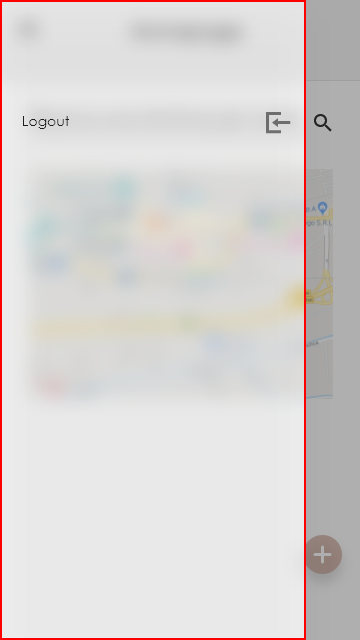
\includegraphics[scale=0.4]{Figures/DrawerUtenteL.png}
    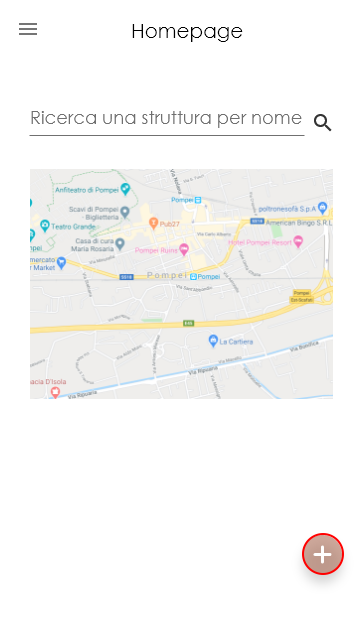
\includegraphics[scale=0.4]{Figures/HomePageUtenteL.png} 
\end{figure}

%%%%% ===============================================================================

